\chapter{Zusammengesetzte Bosonen, Spin-Darstellungen und Dirac-Verdopplung}

\section{Austauschsymmetrie und zusammengesetzte Bosonen}

Die einleitende Frage ist ein echtes Paradoxon zusammengesetzter Teilchen: Wenn zwei Fermionen ein Boson bilden, können dann zwei solche Bosonen denselben Zustand einnehmen, ohne das Pauli-Prinzip zu verletzen? Die Antwort beginnt mit der Austauschsymmetrie selbst.

Nehmen wir an, zwei identische Teilchen werden durch eine Wellenfunktion mit zwei Argumenten beschrieben. Die Symbole \(x\) und \(y\) bezeichnen die beiden Teilchenplätze; sie unterscheiden keine Teilchensorten. Für Bosonen ist die Wellenfunktion symmetrisch, für Fermionen antisymmetrisch:
\begin{equation}
\Psi_B(x,y)=\Psi_B(y,x),
\qquad
\Psi_F(x,y)=-\Psi_F(y,x).
\end{equation}
Die Symmetrie bedeutet, dass der Austausch der beiden ununterscheidbaren Teilchen keinen neuen physikalischen Zustand ergibt.

Zwei Bosonen können durchaus denselben Einteilchenzustand einnehmen. Hat dieser Zustand die Wellenfunktion \(\varphi\), so lautet das Produkt für zwei Teilchen
\begin{equation}
\Psi(x,y)=\varphi(x)\varphi(y).
\end{equation}
Wellenfunktionen sind gewöhnliche komplexwertige Funktionen, keine Operatoren oder Matrizen; daher kommutieren ihre Werte:
\begin{equation}
\varphi(x)\varphi(y)=\varphi(y)\varphi(x).
\end{equation}
Das Produkt ist folglich symmetrisch. Dieselbe Konstruktion kann keinen von null verschiedenen Zustand aus zwei Fermionen ergeben, denn Antisymmetrie würde verlangen:
\begin{equation}
\varphi(x)\varphi(y)=-\varphi(y)\varphi(x),
\end{equation}
während die beiden Seiten ohne das Minuszeichen gleich sind.

Allgemeiner können wir von einer beliebigen Zweiteilchen-Wellenfunktion \(F(x,y)\) ausgehen, für die keine Austauschsymmetrie vorausgesetzt wird. Ihr symmetrischer und ihr antisymmetrischer Anteil lauten bis auf einen Normierungsfaktor
\begin{align}
F_{\mathrm{sym}}(x,y)&=F(x,y)+F(y,x),\\
F_{\mathrm{asym}}(x,y)&=F(x,y)-F(y,x).
\end{align}
Die Überprüfung der Austauschsymmetrie ist unmittelbar:
\begin{align}
F_{\mathrm{sym}}(y,x)
&=F(y,x)+F(x,y)
=F_{\mathrm{sym}}(x,y),\\
F_{\mathrm{asym}}(y,x)
&=F(y,x)-F(x,y)
=-F_{\mathrm{asym}}(x,y).
\end{align}
Durch Addition der ausgetauschten Funktion erhält man die Symmetrisierung, durch Subtraktion die Antisymmetrisierung.

Ein Paar Wasserstoffatome ist der interessantere Fall. Es besteht aus vier fermionischen Bestandteilen: zwei identischen Elektronen und zwei identischen Protonen. Die Elektronenvariablen seien mit \(x_1,x_2\) und die Protonenvariablen mit \(y_1,y_2\) bezeichnet. Die Vierkörper-Wellenfunktion muss sowohl beim Austausch der Elektronen als auch beim Austausch der Protonen jeweils antisymmetrisch sein:
\begin{align}
\Psi(x_2,x_1;y_1,y_2)
&=-\Psi(x_1,x_2;y_1,y_2),\\
\Psi(x_1,x_2;y_2,y_1)
&=-\Psi(x_1,x_2;y_1,y_2).
\end{align}

Um zwei verschiedene Wellenfunktionen für je ein Atom einzuführen, stellen wir uns ein Wasserstoffatom vor, das mit der Wellenfunktion \(\psi(x,y)\) in der Nähe des Ursprungs lokalisiert ist, und ein weiteres, das an einem anderen Ort mit der Wellenfunktion \(\phi(x,y)\) lokalisiert ist. Die zweite kann einfach eine verschobene Kopie der ersten sein, die durch Verschiebung sowohl ihres Elektronen- als auch ihres Protonenarguments entsteht; in dieser Beschreibung ist sie dennoch eine eigene Wellenfunktion. Ein naives Produkt lautet
\begin{equation}
\psi(x_1,y_1)\phi(x_2,y_2).
\end{equation}
Es weist noch keine der beiden erforderlichen fermionischen Antisymmetrien auf.

Zuerst antisymmetrisieren wir die Elektronenvariablen:
\begin{equation}
\Psi_x=
\psi(x_1,y_1)\phi(x_2,y_2)
-\psi(x_2,y_1)\phi(x_1,y_2).
\end{equation}
Unter \(x_1\leftrightarrow x_2\) tauschen die beiden Terme ihre Plätze, und der gesamte Ausdruck wechselt das Vorzeichen. Nun antisymmetrisieren wir dieses Ergebnis bezüglich der Protonenvariablen. Die Reihenfolge der vier Terme ergibt sich aus den beiden aufeinanderfolgenden Antisymmetrisierungen.\footnote{Diese Konstruktion legt auch das Vorzeichenmuster \(+,-,-,+\) fest, das sich aus den Korrekturen der Variablenbezeichnungen während der mündlichen Rechnung ergibt.}
\begin{align}
\Psi_{2H}(x_1,x_2;y_1,y_2)
&=\Psi_x(x_1,x_2;y_1,y_2)\nonumber\\
&\quad{}-\Psi_x(x_1,x_2;y_2,y_1)\\
&=\psi(x_1,y_1)\phi(x_2,y_2)\nonumber\\
&\quad{}-\psi(x_2,y_1)\phi(x_1,y_2)\nonumber\\
&\quad{}-\psi(x_1,y_2)\phi(x_2,y_1)\nonumber\\
&\quad{}+\psi(x_2,y_2)\phi(x_1,y_1).
\label{eq:two-hydrogen-antisymmetrized}
\end{align}
Beim Austausch der Elektronen werden die ersten beiden und die letzten beiden Terme vertauscht, wobei sich das Gesamtvorzeichen umkehrt. Für den Austausch der Protonen gilt dasselbe. Der Zustand besitzt somit genau die beiden separaten Antisymmetrien, die für die fermionischen Bestandteile erforderlich sind.

\begin{classroomqa}
\lecturetimestamp{00:11:11}
\audiencequestion{Wenn Wasserstoffatome Bosonen sind, was hindert uns daran, zwei von ihnen direkt übereinanderzulegen?}
\lecturerresponse{Die bosonische Austauschsymmetrie beseitigt die Kräfte zwischen den Atomen nicht. Das Pauli-Prinzip für die Bestandteile kann zusammen mit den übrigen Wechselwirkungskräften zwischen den Atomen eine räumliche Überlappung extrem kostspielig machen. Das ist eine andere Frage als die, ob die Atome denselben delokalisierten Impulszustand einnehmen dürfen. Ein Impulseigenzustand ist über den gesamten Raum ausgedehnt; gleicher Impuls bedeutet also nicht, die Atome auf denselben Punkt zu rammen. Selbst harte Objekte wie Billardkugeln könnten der bosonischen Austauschsymmetrie gehorchen: Ihre harten Kerne würden eine räumliche Überlappung verhindern, während die bosonische Statistik weiterhin die gemeinsame Besetzung eines Impulszustands zuließe.}
\end{classroomqa}

\begin{classroomqa}
\lecturetimestamp{00:12:28}
\audiencequestion{Würden bei zwei Wasserstoffatomen im selben Impulseigenzustand auch ihre fermionischen Bestandteile denselben Zustand einnehmen?}
\lecturerresponse{Nein. Der Vierkörperzustand bleibt beim Austausch der beiden Elektronenvariablen antisymmetrisch und ebenso separat beim Austausch der beiden Protonenvariablen. Nur der gleichzeitige Austausch beider Bestandteile---also der Austausch der beiden ganzen Atome---ist symmetrisch.}
\end{classroomqa}

Tatsächlich bedeutet der Austausch der beiden Atome, beide Vertauschungen vorzunehmen:
\begin{equation}
x_1\leftrightarrow x_2,
\qquad
y_1\leftrightarrow y_2.
\end{equation}
Die erste Vertauschung liefert ein fermionisches Minuszeichen, die zweite ein weiteres:
\begin{equation}
\begin{aligned}
\Psi_{2H}(x_2,x_1;y_2,y_1)
&=(-1)(-1)\Psi_{2H}(x_1,x_2;y_1,y_2)\\
&=\Psi_{2H}(x_1,x_2;y_1,y_2).
\end{aligned}
\end{equation}
Dasselbe Ergebnis lässt sich Term für Term in Gl.~\eqref{eq:two-hydrogen-antisymmetrized} ablesen. Beim Austausch der ganzen Atome gilt
\begin{equation}
\psi(x_1,y_1)\phi(x_2,y_2)
\longleftrightarrow
\psi(x_2,y_2)\phi(x_1,y_1),
\end{equation}
sodass der erste und der vierte Term vertauscht werden. Ebenso gilt
\begin{equation}
-\psi(x_2,y_1)\phi(x_1,y_2)
\longleftrightarrow
-\psi(x_1,y_2)\phi(x_2,y_1),
\end{equation}
sodass der zweite und der dritte Term vertauscht werden. Der vollständige Zustand ist beim Vertauschen der Atome symmetrisch. Zwei fermionische Minuszeichen ergeben für das zusammengesetzte Teilchen ein Pluszeichen.

Diese Aussage zur Austauschsymmetrie ist logisch unabhängig von der Energie, die für eine Überlappung der Atome erforderlich ist. Eine starke Abstoßung kann eine solche Überlappung unzugänglich machen, ändert aber nichts am symmetrischen Austauschgesetz.

\begin{classroomqa}
\lecturetimestamp{00:14:42}
Was stellt der konstruierte Vierkörperzustand physikalisch dar, und handelt es sich speziell um einen Impulsraumzustand?\audiencequestion{
}\lecturerresponse{Er ist die Wellenfunktion für zwei Atome, die aus zwei Einatom-Wellenfunktionen gebildet wird, indem zuerst die Elektronenbezeichnungen und anschließend die Protonenbezeichnungen antisymmetrisiert werden. Sie muss nicht im Impulsraum formuliert sein. Die Variablen können Positionen, Impulse oder eine andere Darstellung beschreiben; die erforderlichen Austauschsymmetrien der Bestandteile bleiben dieselben.}
\end{classroomqa}

Daher können zwei Atome dieselbe delokalisierte Impulswellenfunktion einnehmen, auch wenn es sehr viel Energie kosten kann, ihre räumlichen Verteilungen zu einer starken Überlappung zu zwingen.

Setzen wir nun die beiden Einatom-Wellenfunktionen gleich, \(\phi=\psi\). Dann wird Gl.~\eqref{eq:two-hydrogen-antisymmetrized} zu
\begin{align}
\Psi_{\mathrm{same}}
&=\psi(x_1,y_1)\psi(x_2,y_2)
-\psi(x_2,y_1)\psi(x_1,y_2)\nonumber\\
&\quad
-\psi(x_1,y_2)\psi(x_2,y_1)
+\psi(x_2,y_2)\psi(x_1,y_1).
\end{align}

Verschwindet dieser Vierkörperzustand? Nein. Das erste und das vierte Produkt sind gleich, ebenso das zweite und das dritte. Wegen der Kommutativität der Einatom-Wellenfunktionen gilt
\begin{equation}
\Psi_{\mathrm{same}}
=
2\left[
\psi(x_1,y_1)\psi(x_2,y_2)
-\psi(x_2,y_1)\psi(x_1,y_2)
\right],
\label{eq:same-hydrogen-state}
\end{equation}
was im Allgemeinen von null verschieden ist. Der Zustand bleibt bezüglich der beiden Elektronenvariablen antisymmetrisch und ebenso separat bezüglich der beiden Protonenvariablen.

Hier wird nicht jeweils ein scharf lokalisiertes Elektron einem scharf lokalisierten Atom zugeordnet. Ein in einem Atom gebundenes Elektron ist über dessen atomare Wellenfunktion räumlich delokalisiert. Haben die beiden Atome denselben Atomzustand, so folgt daraus weder \(x_1=x_2\) noch \(y_1=y_2\).

Die Ausschließung der Bestandteile zeigt sich unmittelbar, wenn wir den Fall gleicher Argumente betrachten. Fallen die beiden modellierten Elektronenargumente zusammen, \(x_1=x_2=x\), so ergibt sich aus Gl.~\eqref{eq:same-hydrogen-state}
\begin{align}
\Psi_{\mathrm{same}}(x,x;y_1,y_2)
&=2\bigl[
\psi(x,y_1)\psi(x,y_2)\nonumber\\
&\quad{}-\psi(x,y_1)\psi(x,y_2)
\bigr]\\
&=0.
\end{align}
Der entsprechende Ausdruck verschwindet auch für \(y_1=y_2\). Die zusammengesetzte Wellenfunktion im gleichen Zustand ist also von null verschieden, während ihre Amplitude für zusammenfallende Argumente identischer Fermionen verschwindet.\footnote{Spin und weitere Einteilchenbezeichnungen sind in diesem Modell unterdrückt. Die fermionische Antisymmetrie gilt für die vollständige Menge der Einteilchenbezeichnungen; die hier gezeigte Auslöschung betrifft das Zusammenfallen der berücksichtigten Argumente.}

\begin{classroomqa}
\lecturetimestamp{00:20:41}
Können die Atome im selben Zustand sein, während sich ihre Elektronen und Protonen nicht in denselben Teilchenzuständen befinden?\audiencequestion{
}\lecturerresponse{Ja. Die Gleichheit der zusammengesetzten atomaren Wellenfunktionen hebt die separaten Antisymmetrien der Elektronen und Protonen nicht auf. Der vollständige Vierkörperzustand kann zwei Atome im selben Atomzustand beschreiben und zugleich für zusammenfallende Argumente identischer Fermionen eine verschwindende Amplitude aufweisen.}
\end{classroomqa}

\begin{classroomqa}
\lecturetimestamp{00:21:12}
Hat die Antisymmetrisierung die Anteile herausprojiziert, bei denen die identischen Bestandteile zusammenfallen?\audiencequestion{
}\lecturerresponse{Ja. In den hier dargestellten Variablen heben sich diese Anteile für zusammenfallende Argumente exakt auf. Präzise gesagt verschwindet die antisymmetrische Wellenfunktion, wenn die beiden Argumente identischer Fermionen gleich sind.}
\end{classroomqa}

Die Auslöschung hängt nicht davon ab, dass die atomaren Wellenfunktionen zuvor gleichgesetzt werden. Für den allgemeinen Zustand aus Gl.~\eqref{eq:two-hydrogen-antisymmetrized} gilt
\begin{align}
\Psi_{2H}(x,x;y_1,y_2)
&=\psi(x,y_1)\phi(x,y_2)\nonumber\\
&\quad{}-\psi(x,y_1)\phi(x,y_2)\nonumber\\
&\quad{}-\psi(x,y_2)\phi(x,y_1)\nonumber\\
&\quad{}+\psi(x,y_2)\phi(x,y_1)\\
&=0.
\end{align}

\begin{classroomqa}
\lecturetimestamp{00:21:32}
Gilt diese Auslöschung auch für Atome in verschiedenen Zuständen, wenn die Argumente identischer Bestandteile zusammenfallen?\audiencequestion{
}\lecturerresponse{Ja. Sie folgt aus der Antisymmetrie selbst, nicht aus der Bedingung \(\phi=\psi\). Dasselbe gilt in einer anderen Darstellung: Nach der Transformation in den Impulsraum verschwindet die Amplitude, wenn die beiden Impulsargumente identischer Fermionen zusammenfallen, vorausgesetzt, auch die übrigen unterdrückten Einteilchenbezeichnungen stimmen überein.}
\end{classroomqa}

\section{Spin als endlichdimensionales Quantensystem}

Die Mathematik des Spins tritt auch beim Isospin, bei der Farbladung und bei den anderen inneren Symmetrien der Teilchenphysik auf. Die Analogie ist formal: Dieselbe Algebra erscheint, auch wenn die physikalischen Größen nicht dieselbe Bedeutung haben müssen. Zunächst wollen wir den Spin etwas weiterentwickeln und danach zur Dirac-Gleichung zurückkehren. Diese mathematischen Mittel werden später auf den Isospin angewandt, ein historisch mit den 1930ern verbundenes Konzept.

Ein Elektron ist ein Spin-\(\tfrac12\)-Teilchen, ebenso wie das Proton und das Myon. Seine Spin-\(z\)-Komponente kann zwei Werte annehmen. Bevor wir die Einheiten festlegen, schreiben wir
\begin{equation}
S_z=m\hbar.
\end{equation}
Von nun an sei \(\hbar=1\). Der Buchstabe \(L\) ist üblicherweise dem Bahndrehimpuls vorbehalten; der intrinsische Spin wird daher mit \(S\) bezeichnet. Er erfüllt dieselbe Drehimpulsalgebra:
\begin{equation}
[S_x,S_y]=iS_z,
\quad
[S_y,S_z]=iS_x,
\quad
[S_z,S_x]=iS_y,
\end{equation}
und
\begin{equation}
S_\pm=S_x\pm iS_y.
\end{equation}
Der Operator \(S_+\) erhöht den \(S_z\)-Eigenwert, und \(S_-\) senkt ihn.

\begin{classroomqa}
\lecturetimestamp{00:25:39}
Geht es hier speziell um den intrinsischen Spin?\audiencequestion{
}\lecturerresponse{Im Mittelpunkt steht der intrinsische Spin. Dieselbe Drehimpulsalgebra gilt allgemeiner, etwa auch für den Bahndrehimpuls oder die Rotation eines makroskopischen Körpers.}
\end{classroomqa}

Für Spin ein halb gibt es nur die \(S_z\)-Eigenwerte \(+\tfrac12\) und \(-\tfrac12\). Lassen wir vorerst alle anderen Eigenschaften des Elektrons außer Betracht: Wir blenden Position und Impuls aus und behalten nur die beiden Spinzustände bei. Dann gilt
\begin{equation}
|\psi\rangle
=
\alpha|\uparrow_z\rangle+\beta|\downarrow_z\rangle
\quad\longleftrightarrow\quad
\begin{pmatrix}
\alpha\\
\beta
\end{pmatrix},
\end{equation}
wobei
\begin{equation}
|\alpha|^2=P(\uparrow_z),
\qquad
|\beta|^2=P(\downarrow_z),
\qquad
|\alpha|^2+|\beta|^2=1.
\end{equation}
Dies ist ein zweidimensionaler Zustandsraum. Damit ist nicht gemeint, dass der gewöhnliche Raum zwei Dimensionen hat.

\begin{classroomqa}
\lecturetimestamp{00:28:18}
Wurde gesagt, der physikalische Raum sei zweidimensional?\audiencequestion{
}\lecturerresponse{Nein. Der Spin-Zustandsraum ist zweidimensional. Position und Impuls wurden vorübergehend ausgeblendet, als wäre das Elektron an eine Wand genagelt und ließe sich nur sein Spin messen.}
\end{classroomqa}

Operatoren auf diesem Zustandsraum werden durch \(2\times2\)-Matrizen dargestellt. Zweckmäßig ist die Wahl der \(S_z\)-Basis, in der \(S_z\) diagonal ist; die Diagonalform ist jedoch eine Basiswahl und keine physikalische Voraussetzung.

\begin{classroomqa}
\lecturetimestamp{00:29:46}
Muss \audiencequestion{ diagonal sein?\(S_z\)
}\lecturerresponse{Nein. Es wird der Einfachheit halber diagonal gewählt. Andere Matrixdarstellungen sind physikalisch gleichwertig.}
\end{classroomqa}

\begin{classroomqa}
\lecturetimestamp{00:30:08}
Ist \audiencequestion{ eine Matrix?\(S_z\)
}\lecturerresponse{\(S_z\) ist eine Observable und daher ein Operator. In der gewählten endlichdimensionalen Basis wird dieser Operator durch eine Matrix dargestellt, die auf Zustandsvektoren wirkt.}
\end{classroomqa}

Eine besonders nützliche Darstellung ist
\begin{equation}
S_i=\frac12\sigma_i,
\end{equation}
wobei
\begin{equation}
\sigma_x=
\begin{pmatrix}
0&1\\
1&0
\end{pmatrix},
\quad
\sigma_y=
\begin{pmatrix}
0&-i\\
i&0
\end{pmatrix},
\quad
\sigma_z=
\begin{pmatrix}
1&0\\
0&-1
\end{pmatrix}.
\end{equation}
Die Matrizen ohne den Faktor ein halb heißen Pauli-Matrizen; die Spinoperatoren selbst enthalten diesen Faktor. Durch direktes Ausmultiplizieren lassen sich die Kommutatorrelationen überprüfen. Die Darstellung ist nicht eindeutig: Eine Drehung der Achsen oder ein Basiswechsel liefert ein anderes, dazu äquivalentes Tripel.

Dies ist eine Darstellung des Drehimpulses mit Spin ein halb durch zweikomponentige Vektoren.

\subsection{Eigenzustände entlang der Koordinatenachsen}

Die Eigenwertgleichungen lassen sich zweckmäßig komponentenweise lösen. Da die Eigenwerte von \(\sigma_i\) gleich \(\pm1\) sind, sind die Eigenwerte von \(S_i=\sigma_i/2\) gleich \(\pm\tfrac12\).

Für \(\sigma_z\) lauten die beiden Gleichungen
\begin{align}
\begin{pmatrix}
1&0\\
0&-1
\end{pmatrix}
\begin{pmatrix}
\alpha\\
\beta
\end{pmatrix}
&=
\begin{pmatrix}
\alpha\\
\beta
\end{pmatrix},
&
\begin{pmatrix}
1&0\\
0&-1
\end{pmatrix}
\begin{pmatrix}
\alpha\\
\beta
\end{pmatrix}
&=
-
\begin{pmatrix}
\alpha\\
\beta
\end{pmatrix}.
\end{align}

\begin{figure}[t]
\centering
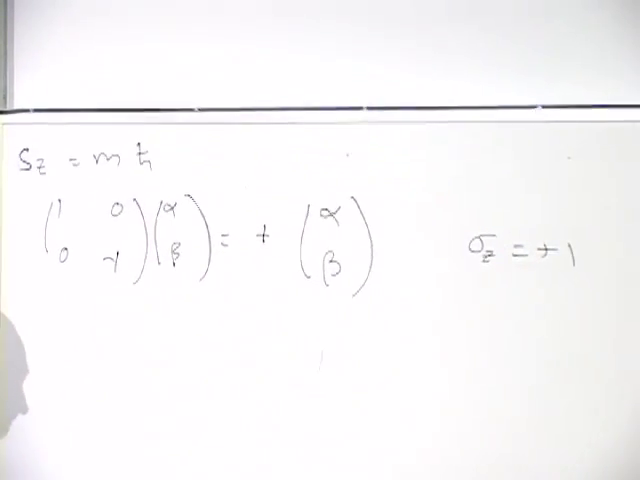
\includegraphics[width=0.74\textwidth]{lecture_08_figure_02.png}
\caption{Die Eigenwertgleichung zum Eigenwert \(+1\) für die Wirkung von \(\sigma_z\) auf einen Zweikomponentenspinor.}
\lectureframe{00:34:57}
\end{figure}

Zum Eigenwert \(+1\) ergibt die zeilenweise Multiplikation
\begin{equation}
\begin{pmatrix}
1\cdot\alpha+0\cdot\beta\\
0\cdot\alpha-\beta
\end{pmatrix}
=
\begin{pmatrix}
\alpha\\
-\beta
\end{pmatrix}
=
\begin{pmatrix}
\alpha\\
\beta
\end{pmatrix}.
\end{equation}
Die obere Gleichung ist automatisch erfüllt, während die untere \(-\beta=\beta\) und damit \(\beta=0\) liefert. Die Normierung verlangt \(|\alpha|=1\). Wählt man die irrelevante Gesamtphase so, dass \(\alpha=1\) gilt, erhält man
\begin{equation}
|+z\rangle=
\begin{pmatrix}
1\\
0
\end{pmatrix}.
\end{equation}

Zum Eigenwert \(-1\) gilt
\begin{equation}
\begin{pmatrix}
\alpha\\
-\beta
\end{pmatrix}
=
\begin{pmatrix}
-\alpha\\
-\beta
\end{pmatrix}.
\end{equation}
Nun ist die untere Gleichung automatisch erfüllt; die obere liefert \(\alpha=-\alpha\), also \(\alpha=0\). Mit der Wahl \(\beta=1\) ergibt sich
\begin{equation}
|-z\rangle=
\begin{pmatrix}
0\\
1
\end{pmatrix}.
\end{equation}

Ändern wir nun das Experiment und messen \(S_x\). Da
\begin{equation}
\sigma_x
\begin{pmatrix}
\alpha\\
\beta
\end{pmatrix}
=
\begin{pmatrix}
0\cdot\alpha+\beta\\
\alpha+0\cdot\beta
\end{pmatrix}
=
\begin{pmatrix}
\beta\\
\alpha
\end{pmatrix},
\end{equation}
lautet die Gleichung zum Eigenwert \(+1\)
\begin{equation}
\begin{pmatrix}
\beta\\
\alpha
\end{pmatrix}
=
\begin{pmatrix}
\alpha\\
\beta
\end{pmatrix}.
\end{equation}
Die beiden Komponentengleichungen \(\beta=\alpha\) und \(\alpha=\beta\) sind dieselbe Bedingung. Aus der Normierung folgt
\begin{equation}
2|\alpha|^2=1,
\end{equation}
Eine zweckmäßige Wahl ist daher
\begin{equation}
|+x\rangle
=
\frac{1}{\sqrt2}
\begin{pmatrix}
1\\
1
\end{pmatrix}.
\end{equation}

\begin{figure}[t]
\centering
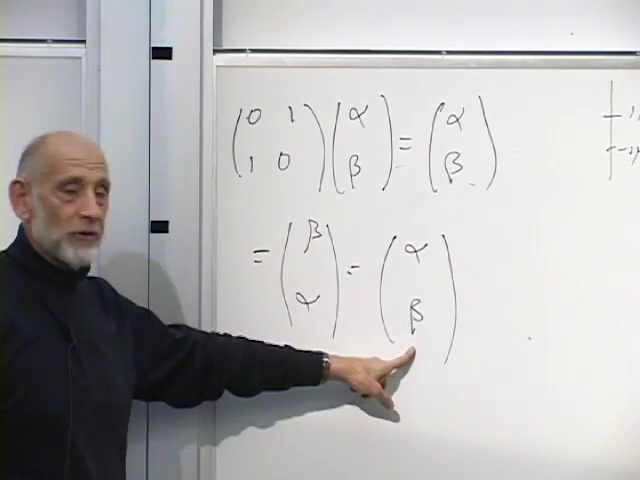
\includegraphics[width=0.74\textwidth]{lecture_08_figure_03.png}
\caption{Zum Eigenwert \(+1\) vertauscht \(\sigma_x\) die beiden Komponenten; daher muss \(\alpha=\beta\) gelten.}
\lectureframe{00:39:42}
\end{figure}

\begin{classroomqa}
\lecturetimestamp{00:40:13}
\audiencequestion{Wenn man den Faktor ein halb einbeziehen würde, wäre der Eigenwert dann ein halb?}
\lecturerresponse{Ja. Die Pauli-Matrix \(\sigma_x\) hat die Eigenwerte \(\pm1\), während \(S_x=\sigma_x/2\) die Eigenwerte \(\pm\tfrac12\) hat.}
\end{classroomqa}

Zum Eigenwert \(-1\) gilt
\begin{equation}
\begin{pmatrix}
\beta\\
\alpha
\end{pmatrix}
=
-
\begin{pmatrix}
\alpha\\
\beta
\end{pmatrix},
\end{equation}
also
\begin{equation}
\beta=-\alpha,
\qquad
\alpha=-\beta.
\end{equation}
Dies ist wiederum dieselbe Gleichung. Nach der Normierung gilt
\begin{equation}
|-x\rangle
=
\frac{1}{\sqrt2}
\begin{pmatrix}
1\\
-1
\end{pmatrix}.
\end{equation}
Eine gleichgewichtete Überlagerung der Zustände \(z\)-auf und \(z\)-ab ist somit entlang der positiven \(x\)-Achse polarisiert; dieselbe Überlagerung mit einem relativen Minuszeichen ist entlang der negativen \(x\)-Achse polarisiert.

Für die Richtung \(y\) gilt
\begin{equation}
\sigma_y
\begin{pmatrix}
\alpha\\
\beta
\end{pmatrix}
=
\begin{pmatrix}
-i\beta\\
i\alpha
\end{pmatrix}.
\end{equation}
Die beiden normierten Eigenvektoren sind
\begin{equation}
|+y\rangle
=
\frac{1}{\sqrt2}
\begin{pmatrix}
1\\
i
\end{pmatrix},
\qquad
|-y\rangle
=
\frac{1}{\sqrt2}
\begin{pmatrix}
1\\
-i
\end{pmatrix},
\end{equation}
bis auf eine Gesamtphase. Beide Zustände ergeben für \(z\)-auf die Wahrscheinlichkeit \(1/2\) und für \(z\)-ab die Wahrscheinlichkeit \(1/2\). Die relative Phase \(i\), die in diesen beiden Wahrscheinlichkeiten nicht sichtbar ist, unterscheidet die \(y\)- von der \(x\)-Polarisation. Linearkombinationen beschreiben auch Spinpolarisationen entlang beliebiger Richtungen; diese Rechnung wird auf später verschoben.

\begin{classroomqa}
\lecturetimestamp{00:44:22}
\audiencequestion{Wurde das Vorzeichen der \(i\)-Komponente dem falschen Eigenwert von \(\sigma_y\) zugeordnet?}
\lecturerresponse{Möglicherweise wurde das Vorzeichen tatsächlich dem falschen Eigenwert zugeordnet. Die Zuordnung ist hier unsicher; sie wird nicht aus dem Gedächtnis festgelegt.}
\end{classroomqa}

Die direkte Überprüfung lautet
\begin{align}
\sigma_y\frac{1}{\sqrt2}
\begin{pmatrix}
1\\
i
\end{pmatrix}
&=
\frac{1}{\sqrt2}
\begin{pmatrix}
-i\,i\\
i
\end{pmatrix}
=
\frac{1}{\sqrt2}
\begin{pmatrix}
1\\
i
\end{pmatrix},\\
\sigma_y\frac{1}{\sqrt2}
\begin{pmatrix}
1\\
-i
\end{pmatrix}
&=
\frac{1}{\sqrt2}
\begin{pmatrix}
(-i)(-i)\\
i
\end{pmatrix}
=
-\frac{1}{\sqrt2}
\begin{pmatrix}
1\\
-i
\end{pmatrix}.
\end{align}
Damit gehört \(+i\) zum Eigenwert \(+1\) und \(-i\) zum Eigenwert \(-1\).\footnote{Auch nach mehreren Korrekturen bleibt die mündliche Zuordnung ungeklärt; die hier gezeigten Vorzeichen ergeben sich aus der dargestellten Matrixmultiplikation.} Jeder Spin-ein-halb-Zustand, einschließlich jedes Zustands mit Polarisation entlang einer beliebigen Richtung, ist eine Linearkombination von \(|+z\rangle\) und \(|-z\rangle\).

\section{Spin eins und ortsabhängige Spinoren}

Für Spin \(1\) sind die möglichen Werte von \(S_z\) \(+1,0,-1\). Der Zustandsraum ist daher dreidimensional. Spin \(1\) ist ganzzahliger Spin und entspricht bosonischer Statistik. Gesucht sind drei \(3\times3\)-Matrizen, die dieselben Drehimpulskommutatoren erfüllen.

Eine Darstellung, die die drei Koordinatenrichtungen gleich behandelt, ist unten angegeben.\footnote{Das Vorzeichen von \(S_y\) ergibt sich aus der bei \(00{:}48{:}50\) sichtbaren Matrix und wird auch durch \([S_x,S_y]=iS_z\) festgelegt. Eine Umkehr dieses Vorzeichens würde den geforderten Kommutator umkehren.}
\begin{equation}
\begin{aligned}
S_x
&=
i
\begin{pmatrix}
0&0&0\\
0&0&1\\
0&-1&0
\end{pmatrix},
&
S_y
&=
i
\begin{pmatrix}
0&0&1\\
0&0&0\\
-1&0&0
\end{pmatrix},\\
S_z
&=
i
\begin{pmatrix}
0&1&0\\
-1&0&0\\
0&0&0
\end{pmatrix}.
\end{aligned}
\end{equation}
Jede Matrix ist \(i\) mal einer reellen antisymmetrischen Matrix. Jede enthält eine \(1\), eine \(-1\) sowie eine verschwindende Zeile und Spalte, die der jeweiligen Koordinate zugeordnet sind: die erste für \(S_x\), die zweite für \(S_y\) und die dritte für \(S_z\). Das ist eine nützliche Eselsbrücke. In dieser Darstellung ist \(S_z\) nicht diagonal.

Sei
\begin{equation}
v=
\begin{pmatrix}
\alpha\\
\beta\\
\gamma
\end{pmatrix}.
\end{equation}
Dann gilt
\begin{equation}
S_zv
=
\begin{pmatrix}
i\beta\\
-i\alpha\\
0
\end{pmatrix}.
\end{equation}
Zum Eigenwert \(+1\) gilt
\begin{equation}
i\beta=\alpha,
\qquad
-i\alpha=\beta,
\qquad
0=\gamma.
\end{equation}
Also \(\beta=-i\alpha\) und \(\gamma=0\). Aus der Normierung folgt \(2|\alpha|^2=1\), somit
\begin{equation}
|m=+1\rangle
=
\frac{1}{\sqrt2}
\begin{pmatrix}
1\\
-i\\
0
\end{pmatrix}.
\end{equation}
Zum Eigenwert \(-1\) gilt
\begin{equation}
i\beta=-\alpha,
\qquad
-i\alpha=-\beta,
\qquad
0=-\gamma,
\end{equation}
also \(\beta=i\alpha\), \(\gamma=0\) und
\begin{equation}
|m=-1\rangle
=
\frac{1}{\sqrt2}
\begin{pmatrix}
1\\
i\\
0
\end{pmatrix}.
\end{equation}
Schließlich ergibt die Gleichung zum Eigenwert null \(\alpha=\beta=0\), sodass \(\gamma\) beliebig bleibt. Die normierte Lösung lautet
\begin{equation}
|m=0\rangle
=
\begin{pmatrix}
0\\
0\\
1
\end{pmatrix}.
\end{equation}
Weitere Eigenwerte gibt es nicht: Diese drei Eigenvektoren spannen den dreidimensionalen Raum vollständig auf. Die Faktoren \(1/\sqrt2\) sind nicht bloß Zierde. Dieselben Koeffizienten gehen später in quantitative experimentelle Vorhersagen ein, wenn die Algebra auf den Isospin angewandt wird.

\begin{classroomqa}
\lecturetimestamp{00:54:10}
\audiencequestion{Wie sind die komplexen Einträge dieser Spin-eins-Eigenvektoren zu lesen?}
\lecturerresponse{Für \(m=+1\) lauten die Komponenten \(1/\sqrt2,-i/\sqrt2,0\), für \(m=-1\) lauten sie \(1/\sqrt2,i/\sqrt2,0\) und für \(m=0\) lauten sie \(0,0,1\).}
\end{classroomqa}

Andere Tripel von Matrizen erfüllen dieselbe Algebra und sind physikalisch gleichwertig. Die obige symmetrische Darstellung ist nützlich, weil sie alle drei Richtungen gleich behandelt; wir werden sie erneut verwenden.

\subsection{Ortsabhängigkeit wieder einführen}

Nun beziehen wir die Bewegung des Teilchens wieder ein. Der Spin kommutiert mit Position und Impuls, daher kann jeweils eine der beiden Größen zusammen mit einer Spin-Komponente festgelegt werden. Position und Impuls kommutieren nicht miteinander; auch verschiedene Spin-Komponenten kommutieren nicht miteinander.

Ein bewegtes Spin-ein-halb-Teilchen wird durch einen ortsabhängigen Spinor beschrieben:
\begin{equation}
\psi(x)=
\begin{pmatrix}
\psi_\uparrow(x)\\
\psi_\downarrow(x)
\end{pmatrix}.
\end{equation}
Die Größen
\begin{equation}
\rho_{\uparrow_z}(x)=|\psi_\uparrow(x)|^2,
\qquad
\rho_{\downarrow_z}(x)=|\psi_\downarrow(x)|^2
\end{equation}
sind gemeinsame Orts- und Spin-Wahrscheinlichkeitsdichten. Ihre Summe
\begin{equation}
\rho(x)=\psi^\dagger(x)\psi(x)
=|\psi_\uparrow(x)|^2+|\psi_\downarrow(x)|^2,
\end{equation}
ist die Ortsdichte. Ist bekannt, dass das Teilchen bei \(x\) nachgewiesen wurde, dann lauten die bedingten Wahrscheinlichkeiten
\begin{equation}
P(\uparrow_z\mid x)
=
\frac{|\psi_\uparrow(x)|^2}{\psi^\dagger(x)\psi(x)},
\qquad
P(\downarrow_z\mid x)
=
\frac{|\psi_\downarrow(x)|^2}{\psi^\dagger(x)\psi(x)},
\end{equation}
vorausgesetzt, \(\rho(x)\neq0\). Ein Elektron wird also durch eine räumliche Wellenfunktion mit zwei Komponenten beschrieben, deren lokale Spinamplituden sich von Ort zu Ort ändern können.

Für ein bewegtes Spin-eins-Teilchen schreiben wir
\begin{equation}
\phi(x)=
\begin{pmatrix}
\phi_1(x)\\
\phi_2(x)\\
\phi_3(x)
\end{pmatrix}.
\end{equation}
An jedem Raumpunkt bilden die drei Komponenten einen Vektor in demselben Spinraum wie zuvor. Teilchen mit Spin eins haben ganzzahligen Spin und sind Bosonen.

\begin{classroomqa}
\lecturetimestamp{01:00:10}
\audiencequestion{Ist \(\phi_1(x)\) selbst die Wahrscheinlichkeit für das Spin-eins-Ergebnis \(m=+1\)?}
\lecturerresponse{Nein. Es ist eine Amplitude in der gewählten dreikomponentigen Basis. Um ein bestimmtes Spinergebnis zu erhalten, bildet man das Bra des entsprechenden normierten Eigenvektors, projiziert das Feld darauf und nimmt den Betrag zum Quadrat.}
\end{classroomqa}

\begin{figure}[t]
\centering
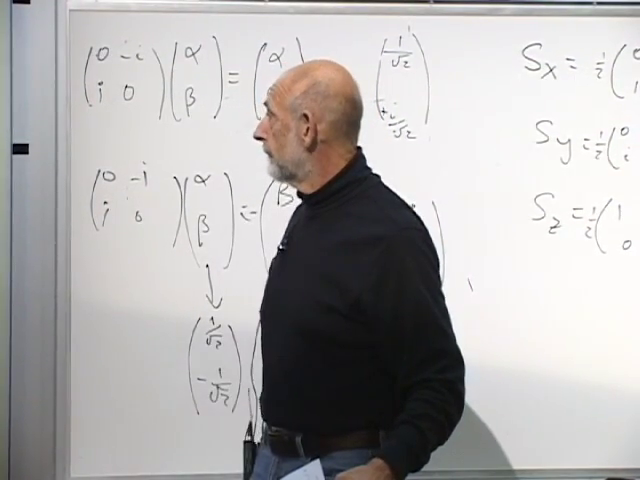
\includegraphics[width=0.82\textwidth]{lecture_08_figure_04.png}
\caption{Normierte Eigenvektoren von \(\sigma_y\) neben den drei Spin-ein-halb-Matrizen.}
\lectureframe{01:00:12}
\end{figure}

Zum Beispiel gilt
\begin{equation}
\begin{aligned}
|m=+1\rangle
&=
\frac{1}{\sqrt2}
\begin{pmatrix}
1\\
-i\\
0
\end{pmatrix}
\\
\Longrightarrow\quad\langle m=+1|
&=
\frac{1}{\sqrt2}
\begin{pmatrix}
1&i&0
\end{pmatrix}.
\end{aligned}
\end{equation}
Die Projektionsamplitude lautet daher
\begin{align}
\langle m=+1|\phi(x)\rangle
&=
\frac{1}{\sqrt2}
\begin{pmatrix}
1&i&0
\end{pmatrix}
\begin{pmatrix}
\phi_1(x)\\
\phi_2(x)\\
\phi_3(x)
\end{pmatrix}\\
&=
\frac{\phi_1(x)+i\phi_2(x)}{\sqrt2}.
\end{align}
Wendet man dieselbe Regel auf alle drei Eigenvektoren an, erhält man die spinaufgelösten Dichten.\footnote{Diese Formeln vervollständigen die Projektionsalgebra nach der ausdrücklichen Korrektur, dass \(\phi_1\) und \(\phi_2\) nicht reell sein müssen. Würde man sie als reell behandeln, ginge die Interferenz fälschlich verloren, die die Dichten für \(m=+1\) und \(m=-1\) unterscheidet.}
\begin{align}
\rho_{+1}(x)
&=
\frac12\left|\phi_1(x)+i\phi_2(x)\right|^2,\\
\rho_{-1}(x)
&=
\frac12\left|\phi_1(x)-i\phi_2(x)\right|^2,\\
\rho_0(x)
&=
|\phi_3(x)|^2.
\end{align}
Sie erfüllen
\begin{equation}
\begin{aligned}
\rho_{+1}(x)+\rho_{-1}(x)+\rho_0(x)
&=
|\phi_1(x)|^2+|\phi_2(x)|^2
\\
&\quad{}+|\phi_3(x)|^2
\\
&=
\phi^\dagger(x)\phi(x).
\end{aligned}
\end{equation}
Ist bekannt, dass das Teilchen bei \(x\) nachgewiesen wurde, dann gilt
\begin{equation}
P(m\mid x)
=
\frac{\rho_m(x)}{\phi^\dagger(x)\phi(x)},
\end{equation}
vorausgesetzt, \(\phi^\dagger(x)\phi(x)\neq0\). Die allgemeine Messregel ist stets dieselbe: Man bildet das Bra des gewünschten normierten Eigenvektors, projiziert den tatsächlichen Zustand darauf und nimmt den Betrag zum Quadrat. Die resultierende Dichte behält ihre Ortsabhängigkeit bei.

Matrizen für höhere Spins sind komplizierter, doch das Prinzip bleibt dasselbe.

\begin{classroomqa}
\lecturetimestamp{01:07:31}
\audiencequestion{Wie groß ist der Zustandsraum für Spin drei halbe?}
\lecturerresponse{Er umfasst vier Zustände mit \(m=\tfrac32,\tfrac12,-\tfrac12,-\tfrac32\). Spin zwei hat fünf Zustände.}
\end{classroomqa}

\begin{classroomqa}
\lecturetimestamp{01:07:55}
\audiencequestion{Warum umfasst die Diskussion \(x,y,z\), aber keine Zeitrichtung? Ist diese Behandlung nichtrelativistisch?}
\lecturerresponse{Bislang ist sie nichtrelativistisch. Spin lässt sich wie die Masse am einfachsten im Ruhesystem des Teilchens charakterisieren; seine Beschreibung in einem anderen Inertialsystem erhält man durch die entsprechende Lorentz-Transformation. Dieser relativistische Schritt wird auf später verschoben.}
\end{classroomqa}

Die Dirac-Gleichung liefert den relativistischen Rahmen und erklärt, warum ihre vierkomponentige Wellenfunktion ein Spin-Dublett enthält.

\section{Dirac-Matrizen und der vierkomponentige Spinor}

Die vierkomponentige Dirac-Wellenfunktion erfüllt
\begin{equation}
i\frac{\partial\Psi}{\partial t}
=
-i\alpha_i\frac{\partial\Psi}{\partial x_i}
+m\beta\Psi,
\qquad i=1,2,3,
\end{equation}
wobei über einen wiederholten räumlichen Index summiert wird. Der Ableitungsterm bedeutet also
\begin{equation}
\alpha_1\frac{\partial\Psi}{\partial x}
+\alpha_2\frac{\partial\Psi}{\partial y}
+\alpha_3\frac{\partial\Psi}{\partial z}.
\end{equation}
Für eine ebene Welle wird daraus die algebraische Gleichung
\begin{equation}
\omega\Psi=(\alpha_i k_i+m\beta)\Psi.
\end{equation}

\begin{classroomqa}
\lecturetimestamp{01:11:32}
\audiencequestion{Bezeichnen die beiden Vorkommen von \(m\) dasselbe?}
\lecturerresponse{Nein. Eines der beiden Vorkommen wurde als räumlicher Index verwendet, das andere bezeichnet die Masse des Teilchens. Benennen wir den räumlichen Index in \(i\) um; tritt \(i\) zweimal auf, wird von \(1\) bis \(3\) summiert.}
\end{classroomqa}

Das Quadrat des Frequenzoperators muss die relativistische Beziehung ergeben:
\begin{equation}
\omega^2=\mathbf{k}^2+m^2.
\end{equation}
Die quadratischen Terme verlangen daher für jedes \(i\)
\begin{equation}
\alpha_i^2=I_4,
\qquad
\beta^2=I_4.
\end{equation}

\begin{classroomqa}
\lecturetimestamp{01:13:01}
\audiencequestion{Ist \(\beta\) für jede der vier Komponenten von \(\Psi\) verschieden?}
\lecturerresponse{Nein. Es gibt eine Matrix \(\beta\), die auf den gesamten vierkomponentigen Spinor wirkt und \(\beta^2=I_4\) erfüllt.}
\end{classroomqa}

Die gemischten Terme müssen verschwinden. Für verschiedene räumliche Richtungen sowie zwischen jedem \(\alpha_i\) und \(\beta\) ergibt sich
\begin{equation}
\alpha_i\alpha_j+\alpha_j\alpha_i=0
\quad (i\neq j),
\qquad
\alpha_i\beta+\beta\alpha_i=0.
\end{equation}
Äquivalent dazu gilt
\begin{equation}
\{\alpha_i,\alpha_j\}=2\delta_{ij}I_4,
\quad
\{\alpha_i,\beta\}=0,
\quad
\{\beta,\beta\}=2I_4.
\end{equation}
Jede Matrix antikommutiert mit jeder anderen Matrix; ihr Antikommutator mit sich selbst ist dagegen das Doppelte der Einheitsmatrix.

Ohne \(\beta\) würden die drei Pauli-Matrizen bereits drei \(2\times2\)-Matrizen liefern, deren Quadrat die Einheitsmatrix ist und die paarweise antikommutieren. Der Massenterm verlangt eine vierte solche Matrix. Es gibt keine vierte \(2\times2\)-Matrix mit den geforderten Eigenschaften, und auch \(3\times3\)-Matrizen erfüllen die Algebra nicht. Die kleinste Darstellung ist daher \(4\times4\).

Eine \(4\times4\)-Matrix lässt sich in vier \(2\times2\)-Blöcke aufteilen. Eine zweckmäßige Darstellung ist
\begin{equation}
\alpha_i=
\begin{pmatrix}
\sigma_i&0\\
0&-\sigma_i
\end{pmatrix},
\qquad i=1,2,3.
\end{equation}

\begin{figure}[t]
\centering
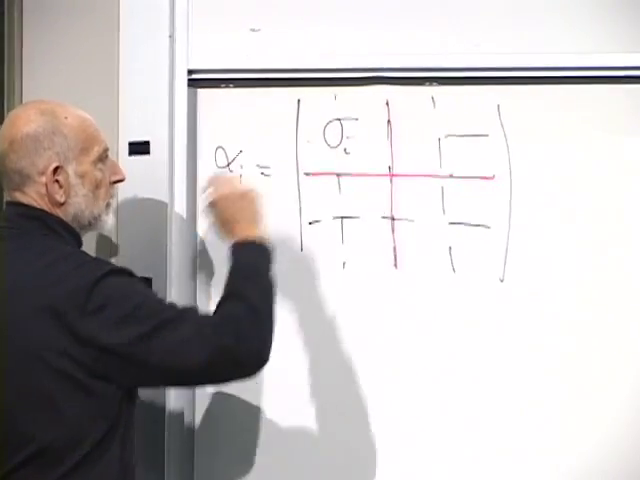
\includegraphics[width=0.68\textwidth]{lecture_08_figure_05.png}
\caption{Die Dirac-Matrix \(\alpha_i\) in \(2\times2\)-Blöcken, mit \(\sigma_i\) und \(-\sigma_i\) auf der Diagonalen.}
\lectureframe{01:17:23}
\end{figure}

\begin{classroomqa}
\lecturetimestamp{01:17:41}
\audiencequestion{Waren die \(\sigma_i\)-Blöcke in der früheren Darstellung anders angeordnet?}
\lecturerresponse{Ja. In einer anderen Darstellung standen sie außerhalb der Diagonalen. Die beiden Anordnungen sind äquivalent und durch eine Ähnlichkeitstransformation miteinander verbunden.}
\end{classroomqa}

In der vorliegenden Darstellung lautet die verbleibende Matrix
\begin{equation}
\beta=
\begin{pmatrix}
0&I_2\\
I_2&0
\end{pmatrix},
\qquad
I_2=
\begin{pmatrix}
1&0\\
0&1
\end{pmatrix}.
\end{equation}
Durch Blockmultiplikation lassen sich Überprüfungen der \(4\times4\)-Algebra auf gewöhnliche Multiplikationen von \(2\times2\)-Matrizen zurückführen.

\begin{classroomqa}
\lecturetimestamp{01:19:17}
\audiencequestion{Verwendete die frühere Darstellung ein anderes Vorzeichen oder eine Diagonalform für \(\beta\)?}
\lecturerresponse{Sie verwendete eine andere, aber physikalisch äquivalente Basis. Ein Basiswechsel mischt die vier Komponenten von \(\Psi\) und verändert das Aussehen der Matrizen, ohne die Physik zu ändern.}
\end{classroomqa}

Die vier Einträge von \(\Psi\) sind nicht die vier Raumzeitkoordinaten. Sie sind Koordinaten im kleinsten Vektorraum, auf dem diese Antikommutationsalgebra wirken kann. Es gibt zwei verschiedene Zweierstrukturen: die Aufteilung in \(2\times2\)-Blöcke und die Zweikomponenten-Pauli-Struktur innerhalb jedes Blocks. Der weiter unten begründeten Deutung vorgreifend lassen sich die vier Möglichkeiten wie folgt anordnen:
\begin{equation}
\begin{array}{c|cc}
& S_z=+\tfrac12 & S_z=-\tfrac12\\ \hline
\omega>0 & (\omega>0,+\tfrac12) & (\omega>0,-\tfrac12)\\
\omega<0 & (\omega<0,+\tfrac12) & (\omega<0,-\tfrac12)
\end{array}.
\end{equation}
Die untere Zeile besteht aus Elektronenzuständen mit negativer Frequenz. Sie ist keine Zeile von Positronen; ein Positron wird als Loch in der gefüllten Menge dieser Zustände gedeutet.

\section{Energieverdopplung im Ruhesystem und das Positron}

Die zweifache Energiestruktur lässt sich am einfachsten bei verschwindendem Impuls sichtbar machen. Wenn \(\mathbf{k}=0\), ist der Zustand der ebenen Welle räumlich konstant und der räumliche Ableitungsterm verschwindet. Die Gleichung im Ruhesystem\footnote{Der Frame bei \(01{:}23{:}38\) enthält auf dem Massenterm vorübergehend noch einen zusätzlichen Faktor \(i\); die mündliche Korrektur bei \(01{:}24{:}05\) entfernt ihn.} lautet
\begin{equation}
i\frac{\partial\Psi}{\partial t}=m\beta\Psi.
\end{equation}

\begin{figure}[t]
\centering
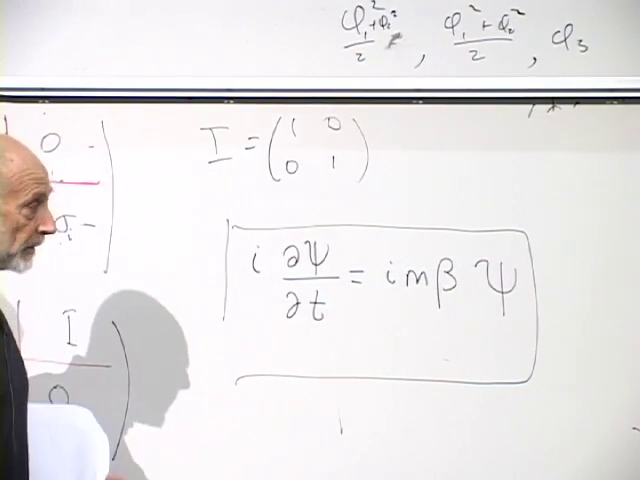
\includegraphics[width=0.76\textwidth]{lecture_08_figure_06.png}
\caption{Bei verschwindendem Impuls verschwinden die räumlichen Ableitungen; übrig bleibt die korrigierte Gleichung im Ruhesystem \(i\partial_t\Psi=m\beta\Psi\).}
\lectureframe{01:23:38}
\end{figure}

Teilen wir die vierkomponentige Spalte in ein oberes und ein unteres zweikomponentiges Objekt auf:
\begin{equation}
\Psi=
\begin{pmatrix}
\psi_+\\
\psi_-
\end{pmatrix}.
\end{equation}

\begin{classroomqa}
\lecturetimestamp{01:24:47}
\audiencequestion{Bedeuten die Bezeichnungen \(\psi_+\) und \(\psi_-\) bereits positive und negative Energie?}
\lecturerresponse{Nein. In diesem Stadium sind es lediglich Namen für den oberen und den unteren Zweikomponentenblock. Ihre Energiekombinationen wurden noch nicht bestimmt.}
\end{classroomqa}

\begin{classroomqa}
\lecturetimestamp{01:25:10}
\audiencequestion{Was stellt die aufgeteilte Spalte mit vier Komponenten dar?}
\lecturerresponse{Es ist derselbe vierkomponentige Dirac-Spinor, angeordnet passend zur Blockform der Matrizen. Jede Hälfte ist ein Objekt mit zwei Komponenten, und zusammen bilden die beiden Objekte die ursprüngliche Spalte mit vier Komponenten.}
\end{classroomqa}

Die Matrix \(\beta\) vertauscht die beiden Blöcke:
\begin{equation}
\beta
\begin{pmatrix}
\psi_+\\
\psi_-
\end{pmatrix}
=
\begin{pmatrix}
\psi_-\\
\psi_+
\end{pmatrix}.
\end{equation}
Damit wird die Gleichung im Ruhesystem zu
\begin{equation}
i\frac{\partial\psi_+}{\partial t}=m\psi_-,
\qquad
i\frac{\partial\psi_-}{\partial t}=m\psi_+.
\end{equation}

Es bieten sich zwei naheliegende Möglichkeiten an. Eine weitere Zeitableitung würde das System entkoppeln, aber durch Addieren und Subtrahieren der beiden Gleichungen wird es unmittelbar diagonalisiert. Tatsächlich gilt
\begin{align}
i\frac{\partial}{\partial t}(\psi_++\psi_-)
&=m(\psi_++\psi_-),\\
i\frac{\partial}{\partial t}(\psi_+-\psi_-)
&=-m(\psi_+-\psi_-).
\end{align}
Mit den Definitionen
\begin{equation}
\chi_+=\psi_++\psi_-,
\qquad
\chi_-=\psi_+-\psi_-,
\end{equation}
erhält man zwei voneinander unabhängige Gleichungen:
\begin{equation}
i\partial_t\chi_+=m\chi_+,
\qquad
i\partial_t\chi_-=-m\chi_-.
\end{equation}
Bei einer Frequenzabhängigkeit der Form \(e^{-i\omega t}\) gilt für die Summe
\begin{equation}
\omega=+m,
\end{equation}
während für die Differenz gilt
\begin{equation}
\omega=-m.
\end{equation}
Das ist genau die Aufspaltung in positive und negative Energie, die wir bereits im früheren eindimensionalen Beispiel gefunden haben: Auch die relativistische Gleichung besitzt Lösungen für Elektronen mit positiver und mit negativer Energie. Die Aufspaltung des Blocks führt also zu Zweigen positiver und negativer Energie. Zustände im reinen Ruhesystem lassen sich schreiben als
\begin{equation}
\Psi_{\omega=+m}=
\begin{pmatrix}
\xi\\
\xi
\end{pmatrix},
\qquad
\Psi_{\omega=-m}=
\begin{pmatrix}
\xi\\
-\xi
\end{pmatrix},
\end{equation}
wobei \(\xi\) weiterhin ein beliebiges Objekt mit zwei Komponenten ist.

Die Summe und die Differenz haben eine der beiden zweifachen Strukturen aufgelöst; die beiden Komponenten von \(\xi\) bleiben jedoch erhalten. Die Pauli-Matrizen wirken auf dieses verbleibende Komponentenpaar. Es ist das mit dem Spin verbundene Paar, was noch anhand von Drehungen und Erhaltungssätzen überprüft werden muss.

\begin{classroomqa}
\lecturetimestamp{01:32:23}
\audiencequestion{Kann man den Spin als äußere zweifache Struktur und das Vorzeichen der Energie als innere auffassen?}
\lecturerresponse{Ja. Die beiden Anordnungen der Faktoren sind gleichwertig. Man kann vertauschen, welcher Index zuerst geschrieben wird; dadurch werden lediglich die vier Komponenten umgeordnet.}
\end{classroomqa}

Der Zweig negativer Frequenz führt zur Interpretation des Dirac-Sees. Einer negativen Frequenz wird eine negative Elektronenenergie zugeordnet. Besetzt man alle Elektronenzustände mit negativer Energie, sinkt die Energie so weit, wie es das Ausschlussprinzip zulässt, denn jeder vollständige fermionische Zustand kann nur von einem Elektron besetzt werden. Das vollständig gefüllte negative Energie-See wird dann als Vakuum bezeichnet.

Man hebt ein Elektron aus diesem gefüllten See in einen Zustand positiver Energie. Das Ergebnis besteht aus einem Elektron mit positiver Energie und einem unbesetzten Zustand negativer Energie. Entfernt man eine negative Energie, steigt die Energie; das Loch hat daher eine positive Anregungsenergie. Da ein Elektron fehlt, trägt es außerdem die entgegengesetzte elektrische Ladung. Das Loch ist ein Positron.

\begin{classroomqa}
\lecturetimestamp{01:32:57}
\audiencequestion{Können Sie die Interpretation des Positrons noch einmal erklären?}
\lecturerresponse{Die Summe der beiden Blöcke hat eine positive Frequenz, die Differenz eine negative. Die Lösungen mit negativer Frequenz sind Elektronenzustände mit negativer Energie, und das Vakuum erhält man, indem man sie alle besetzt. Hebt man ein besetztes Elektron in einen Zustand positiver Energie, bleiben sowohl ein Elektron mit positiver Energie als auch ein Loch zurück. Dieses Loch mit positiver Energie und entgegengesetzter Ladung ist das Positron.}
\end{classroomqa}

Die Algebra hat somit zugleich zwei Folgen hervorgebracht: Zweige positiver und negativer Energie, aus denen die Teilchen--Antiteilchenstruktur entsteht, und eine verbleibende Zweikomponentenstruktur, die mit dem Spin eins halb verbunden ist. Bemerkenswert ist, dass beides aus den kleinsten Matrizen hervorging, die die relativistischen Antikommutationsrelationen erfüllen können. Der Spin war erst kurz zuvor als empirische Eigenschaft entdeckt worden, als diese mathematische Konstruktion Teilchen mit Spin und zugleich einen Antiteilchenzweig hervorbrachte; im damaligen historischen Kontext war das ein dramatisches Ergebnis.

\begin{classroomqa}
\lecturetimestamp{01:35:14}
\audiencequestion{Sind die Elektronen mit negativer Energie selbst Positronen?}
\lecturerresponse{Nein. Die Elektronenzustände mit negativer Energie sind im Vakuum besetzt. Ein Positron ist das Fehlen eines Elektrons in dieser besetzten Menge: ein Loch, kein Elektron mit negativer Energie.}
\end{classroomqa}

Ein Loch kann an Übergängen beteiligt sein. Ein Positron hat positive Energie, weil es dem Fehlen eines Elektrons mit negativer Energie entspricht. Füllt ein Elektron mit positiver Energie das Loch, annihilieren Elektron und Positron; ihre Energie muss jedoch abgeführt werden, gewöhnlich durch Photonen. In der Sprache des Dirac-Sees hat ein Elektron einen unbesetzten Zustand negativer Energie besetzt. Dieselbe Energiefreisetzung lässt sich als Übergang eines angeregten Elektrons in einem Atom auf ein niedrigeres Energieniveau veranschaulichen: Beim Übergang nach unten werden Photonen emittiert.

\begin{classroomqa}
\lecturetimestamp{01:36:39}
\audiencequestion{Warum fallen Elektronen mit höherer negativer Energie nicht in das Loch?}
\lecturerresponse{Diese Frage vermischt zwei Fälle. Wenn ein Elektron mit positiver Energie das Loch füllt, kommt es zur Elektron--Positron-Annihilation; Photonen tragen die Energie fort. Ein Übergang durch ein Elektron aus dem See mit negativer Energie ist ein anderer Prozess, der weiter unten behandelt wird.}
\end{classroomqa}

Die Rechnung für verschwindenden Impuls hat für sich genommen gezeigt, dass nach Abtrennung des Energievorzeichens eine zweifache Entartung verbleibt. Eine Entartung zweier Zustände ist für sich allein kein Beweis dafür, dass diese Zustände Drehimpuls tragen.

\begin{classroomqa}
\lecturetimestamp{01:37:44}
\audiencequestion{Wie beweist die Rechnung für verschwindenden Impuls, dass das verbleibende Zuständepaar den Spin darstellt?}
\lecturerresponse{Man kann das Paar als Spin-auf und Spin-ab bezeichnen, und in der vollständigen Gleichung treten die Pauli-Matrizen auf; das allein ist aber noch kein Beweis. Man muss entweder zeigen, wie sich das Paar unter räumlichen Drehungen transformiert, oder nachweisen, dass bei der Zuordnung eines Spins der Gesamtdrehimpuls in Wechselwirkungen und Stößen erhalten bleibt. Dieser Nachweis folgt später.}
\end{classroomqa}

Für einen Zustand positiver Energie im Ruhesystem sind der obere und der untere Block gleich:
\begin{equation}
\Psi_{\omega=+m}=
\begin{pmatrix}
\xi\\
\xi
\end{pmatrix}.
\end{equation}
Dass \(\xi\) ein Drehimpulsdublett bildet, muss durch das soeben beschriebene Drehungs- oder Erhaltungsargument nachgewiesen werden; es folgt nicht allein daraus, dass zwei Komponenten vorhanden sind.

\begin{classroomqa}
\lecturetimestamp{01:40:46}
\audiencequestion{Kann ein anderes Elektron mit dem Positron annihilieren, auch wenn es eine andere Energie hat?}
\lecturerresponse{Ja. Elektronen behalten keine individuelle Identität. Jedes verfügbare Elektron kann das Loch füllen; Unterschiede in der anfänglichen Energie und im anfänglichen Impuls spiegeln sich in Anzahl und Energien der emittierten Photonen wider.}
\end{classroomqa}

Das Lochbild erklärt auch einen Übergang, der vollständig innerhalb des negativen Energie-Sees abläuft. Angenommen, ein besetzter Zustand mit negativer Energie geht in das Loch über. Das ursprüngliche Loch wird gefüllt, aber der Zustand, aus dem dieses Elektron kam, ist nun leer. Das Loch hat sich verschoben. Gleichbedeutend damit hat das Positron seine Energie geändert und Strahlung emittiert.

\begin{classroomqa}
\lecturetimestamp{01:42:12}
\audiencequestion{Warum können benachbarte Energieniveaus mit negativer Energie nicht nacheinander in das Loch fallen?}
\lecturerresponse{Sie können das Loch von einem Niveau zu einem anderen verschieben. Ein Elektron, das in das ursprüngliche Loch fällt, hinterlässt an seiner vorherigen Energie ein neues Loch; so erhält das ursprüngliche Positron eine andere Energie. Die Energiedifferenz wird von Photonen fortgetragen.}
\end{classroomqa}

\begin{classroomqa}
\lecturetimestamp{01:44:39}
\audiencequestion{Warum führt dies nicht zu einer endlosen Strahlungskaskade zu immer niedrigeren Energien?}
\lecturerresponse{Weil Energie und Impuls gleichzeitig erhalten bleiben müssen. Diese beiden Erhaltungssätze lassen den uneingeschränkten Prozess nicht zu. Dasselbe gilt für ein gewöhnliches freies Elektron: Es kann nicht einfach im leeren Raum fortwährend seine Energie senken, indem es Photonen emittiert.}
\end{classroomqa}
